 \chapter[The 23$^{\text{d}}$ of May 2024 - Proper residual \& strategy]{Proper residual \& strategy}

\begin{chapabstract}
	Meeting report
\end{chapabstract}


\minitoc

\section{Proper residual}

When assessing the loss residual on the continuous interpolated solution, the discretisation error pollutes the loss term. It can thus be interesting to remove its contribution to the loss by restricting the test functions to functions living in the space spanned by the shape functions used for the FE interpolation.

The objective is therefore to minimise the residual
\begin{equation}
	\mathcal{R} = - \int_{\Omega} \eps\left(\vect{u}\right):\ftensor{K}:\vect{u^*} \d \Omega + \int_{\Omega} \vect{f}\cdot \vect{u^*}\d \Omega, \forall \vect{u^* \in \text{Span}\left(\left\{N_i\left(\vect{x}\right)\right\}_{i\in \llbracket 1,n \rrbracket}\right)}
\end{equation}

\section{Parametrisation}

In order to decrease the number of parameters required to parametrised the surrogate model (Shape of the lung, porosity field, etc.) an auto-encoder can be used to get a reduced number of parameter in a latent space that would then be fed as input parameters of the surrogate model as shown in \cref{fig:autoencoderHiDeNNPGD}

Let the input layer be composed of the fields from the scan, \emph{i.e.}

\begin{equation}
	\vect{\Psi} = \begin{pmatrix}
		\vect{\phi} \\  
		\vect{E}\\  
		\vect{\rho}    
	\end{pmatrix}, 
\end{equation}
with $\vect{\phi} $ the morphing between the scanned geometry and the nominal lung geometry on which the computations are performed, $\vect{E}$ the stifness field and $\vect{\rho}$ the density field. 


\begin{figure}
\centering
	% \tikzsetnextfilename{HiDeNN_MultiP}
		\begin{neuralnetwork}[height=8]
	\tikzstyle{input neuron}=[neuron, fill=GreenLMS, text=white];
	\tikzstyle{output neuron}=[neuron, fill=accentcolor, text=white];
	\tikzstyle{hidden neuron}=[neuron, draw = LGreenLMS, thick, fill=LGreenLMS!25, text=LGreenLMS!60!black];
	
	\inputlayer[count=8, bias=false, title=Input Layer, text=\xin]
	
	\hiddenlayer[count=5, bias=false]
	\linklayers
	
	\hiddenlayer[count=3, bias=false, title=Latent space \\ $\left\{\mu_i\right\}_{i=\llbracket 1, \beta \rrbracket}$,text=\xhid]
	\linklayers
	
	\hiddenlayer[count=5, bias=false]
	\linklayers
	
	\outputlayer[count=8, title=Output Layer, text=\xout]
	\linklayers
	
\end{neuralnetwork}
	\caption{Autoencoder for the field parameters}
	\label{fig:autoencoder}
\end{figure}


\begin{figure}[H]
	\centering
	\includegraphics[width = 0.8\linewidth]{Schema/AutoencoderHiDeNNPGD.pdf}
	\caption{Fully parametrised architecture}
	\label{fig:autoencoderHiDeNNPGD}
\end{figure}

\Rq{Put only a binary classification of stifness regions in the lattent space and keep the stifness value in the explicit parametrisation.}

\Rq{Does it make sens to train directly the fully parametrised architecture instead of first training the autoencoder and then the HiDeNN-PGD?}